\chapter{Loop tree \Author{S. Pop}}
\inputprogress
\graphicspath{{fig/}{loop_tree/fig/}{part3/loop_tree/fig/}}


\providecommand{\SSA}{SSA}
\providecommand{\CFG}{CFG}
\providecommand{\loopphi}{loop-$\phi$}
\providecommand{\closephi}{close-$\phi$}
\providecommand{\CHREC}[1]{\{#1\}}

This chapter presents an extension of the \SSA{} under which the
extraction of the reducible loop tree can be done only on the \SSA{}
graph itself.  This extension of the \SSA{} representation captures
more than the scalar computations: the phi nodes and the scalar
assignments encode the structure of the CFG and the strongly connected
components of the CFG that are the reducible natural loops.  This
chapter will present two analysis algorithms: the extraction of the
reducible loop tree and the analysis of induction variables based on
the \SSA{} representation.

\section{\CFG{} and Loop Tree can be discovered from the \SSA{}}

During the construction of the \SSA{} representation based on a \CFG{}
representation, a large part of the \CFG{} information is translated
into the \SSA{} representation.  As the construction of the \SSA{} has
precise rules to place the phi nodes in special points of the \CFG{}
(i.e., at the merge of control-flow branches), by identifying patterns
of uses and definitions, it is possible to expose the \CFG{} structure
from the \SSA{} representation.

Furthermore, it is possible to identify, based on the \SSA{}
definitions and uses patterns, higher level constructs inherent to the
\CFG{} representation, such as strongly connected components of basic
blocks (or natural loops).  The induction variable analysis, that we
will see in this chapter, is based on the detection of self references
in the \SSA{} representation, and on the characterization of these
cyclic definitions.

This first section shows that the classical \SSA{} representation is
not enough to represent the semantics of the original program.  We
will see the minimal amount of information that has to be added to the
classical \SSA{} representation in order to represent the loop
information in an elegant way: the loop closed \SSA{} form adds an
extra variable at the end of a loop for each variable defined in a
loop and used after the loop.  This is similar to the Gated \SSA{}
form presented in Chapter~\ref{chap:vsdg}.

\subsection{An \SSA{} representation without the \CFG{}}

In the classic definition of the \SSA{}, the \CFG{} provides the
skeleton of the program: basic blocks contain assignment statements
defining \SSA{} variable names, and the basic blocks with multiple
predecessors contain phi nodes.  Let's look at what happens when,
starting from a classic \SSA{} representation, we remove the \CFG{}.

In order to remove the \CFG{}, a pretty printer function writes the
content of basic blocks by traversing the \CFG{} structure (the \CFG{}
traversal could be performed in any order: random order, depth-first
order, dominator order, etc.).  Does the representation, obtained from
this pretty printer, contain enough information to enable us to
compute the same thing as the original program?

Let's see what happens with an example: supposing that the original
program looks like this (in its \CFG{} based \SSA{} representation):
\begin{verbatim}
bb_1 (preds = {bb_0}, succs = {bb_2})
{
  a = #some computation independent of b
}
bb_2 (preds = {bb_1}, succs = {bb_3})
{
  b = #some computation independent of a
}
bb_3 (preds = {bb_2}, succs = {bb_4})
{
  c = a + b;
}
bb_4 (preds = {bb_3}, succs = {bb_5})
{
  return c;
}
\end{verbatim}
after removing the \CFG{} structure, using a random order traversal,
we could obtain this:
\begin{verbatim}
  return c;
  b = #some computation independent of a
  c = a + b;
  a = #some computation independent of b
\end{verbatim}
and this \SSA{} code is enough, in the absence of side effects, to
recover an order of computation that leads to the same result as in
the original program.  For example, the evaluation of this sequence of
statements would produce the same result:
\begin{verbatim}
  b = #some computation independent of a
  a = #some computation independent of b
  c = a + b;
  return c;
\end{verbatim}

\subsection{Discovering natural loop structures on the \SSA{}}
We will now see how to represent the natural loops in the \SSA{} form
by systematically adding extra phi nodes at the end of loops, together
with extra information about the loop exit predicate.

Supposing that the original program contains a loop:
\begin{verbatim}
bb_1 (preds = {bb_0}, succs = {bb_2})
{
  x = 3;
}
bb_2 (preds = {bb_1, bb_3}, succs = {bb_3, bb_4})
{
  i = phi (x, j)
  if (i < N) goto bb_3 else goto bb_4;
}
bb_3 (preds = {bb_2}, succs = {bb_3})
{
  j = i + 1;
}
bb_4 (preds = {bb_2}, succs = {bb_5})
{
  k = phi (i)
}
bb_5 (preds = {bb_4}, succs = {bb_6})
{
  return k;
}
\end{verbatim}
Pretty printing, with a random order traversal, we could obtain this
\SSA{} code:
\begin{verbatim}
  x = 3;
  return k;
  i = phi (x, j)
  k = phi (i)
  j = i + 1;
\end{verbatim}
We can remark that some information is lost in this pretty printing:
the exit condition of the loop disappeared: we will have to record
this information in the extension of the \SSA{} representation.  The
information about the natural loop is still available under the form
of a cyclic definition: by simple substitutions, we can rewrite this
\SSA{} code to expose the self reference to ``i'', as:
\begin{verbatim}
  i = phi (3, i + 1)
  k = phi (i)
  return k;
\end{verbatim}
Thus, we have the definition of the \SSA{} name ``i'' defined in
function of itself.  This pattern is characteristic of the existence
of a natural loop.  We can remark that there are two kinds of phi
nodes used in this example:
\begin{itemize}
\item \loopphi{} nodes ``i = phi (x, j)'' have an invariant argument
  ``x'' (i.e., the definition does not depend on the values that the
  phi node takes) and an argument that contains a self reference ``j''
  (i.e., the defining expression ``j = i + 1'' contains a reference to
  the same \loopphi{} definition ``i'').  It is possible to define a
  canonical \SSA{} form by limiting the number of arguments of
  \loopphi{} nodes to two.
\item \closephi{} nodes ``k = phi (i)'' merge the values in the end of
  a loop.  They are used to capture the last value of a name defined
  in a loop.  Names defined in a loop can only be used within that
  loop or in the arguments of a \closephi{} node (that is ``closing''
  the set of uses of the names defined in that loop).  In a canonical
  \SSA{} form it is possible to limit the number of arguments of
  \closephi{} nodes to one.
\end{itemize}

\subsection{Improving the \SSA{} pretty printer for loops}

As we have seen in the above example, the exit condition of the loop
disappears during the basic pretty printing of the \SSA{}.  To capture
the semantics of the computation of the loop, we have to specify in
the \closephi{} node, which value will be available in the end of the
loop.  And thus we have to slightly modify the syntax of the
\closephi{} nodes to also contain the loop exit condition.  This
representation is also known under the name of Gated \SSA{}, as
presented in Chapter~\ref{chap:vsdg}.  With this extension, the
\SSA{} pretty printing of the above example would be:
\begin{verbatim}
  x = 3;
  i = loop-phi (x, j)
  j = i + 1;
  k = close-phi (i >= N, i)
  return k;
\end{verbatim}
So ``k'' is defined as the first value of ``i'' satisfying the loop
exit condition, ``i $>=$ N''.  This is a well defined value (in the
case of finite loops), as the sequence of values that ``i'' takes, is
defined by the \loopphi{} node and taking the first element of that
sequence satisfying the loop exit condition.

In the next section, we will look at an algorithm that translates the
\SSA{} representation into a representation of polynomial functions,
describing the sequence of values that \SSA{} names take during the
execution of a loop.

\section{Analysis of Induction Variables}

The purpose of the induction variables analysis is to provide a
characterization of the sequences of values taken by a variable during
the execution of a loop.  This characterization can be an exact
function of the iteration counter of the loop (i.e., the canonical
induction variable of a loop starts at zero with a step of one for
each iteration of the loop) or an approximation of the values taken
during the execution of the loop represented by values in an abstract
domain.  In this section, we will see a possible characterization of
induction variables in terms of scalar sequences.  The domain of
scalar sequences will be represented by the chains of recurrences: as
we will see in more detail in this section, the canonical induction
variable will be syntactically represented by the chain of recurrence
$\CHREC{0, +, 1}_x$ the initial value of the canonical induction
variable is $0$, the stride is $1$, and the evolution happens in loop
number $x$.

\subsection{Stride detection}

The first step of the induction variables analysis is the detection of
the strongly connected components of the \SSA{}.  This can be
performed by traversing the \SSA{} chains (from a use to its unique
definition) and detecting that some definitions are visited twice.
From a self referring use-def chain, it is possible to compute the
overall effect of one iteration of the loop on the cyclic definition:
this is the step of the induction variable.  When the step of an
induction variable depends on another cyclic definition, one has to
further analyze the inner cycle.  The analysis of the induction
variable ends when all the inner cyclic definitions used for the
computation of the step are analyzed.  Note that it is possible to
construct \SSA{} graphs with strongly connected components that are
impossible to characterize with the chains of recurrences.  For
example, in the following example, ``a'' does not follow a linear
progression:
\begin{verbatim}
  a = loop-phi (0, b)
  c = loop-phi (1, d)
  b = c + 2
  d = a + 3
\end{verbatim}

\begin{figure}[h]
  \begin{center}
    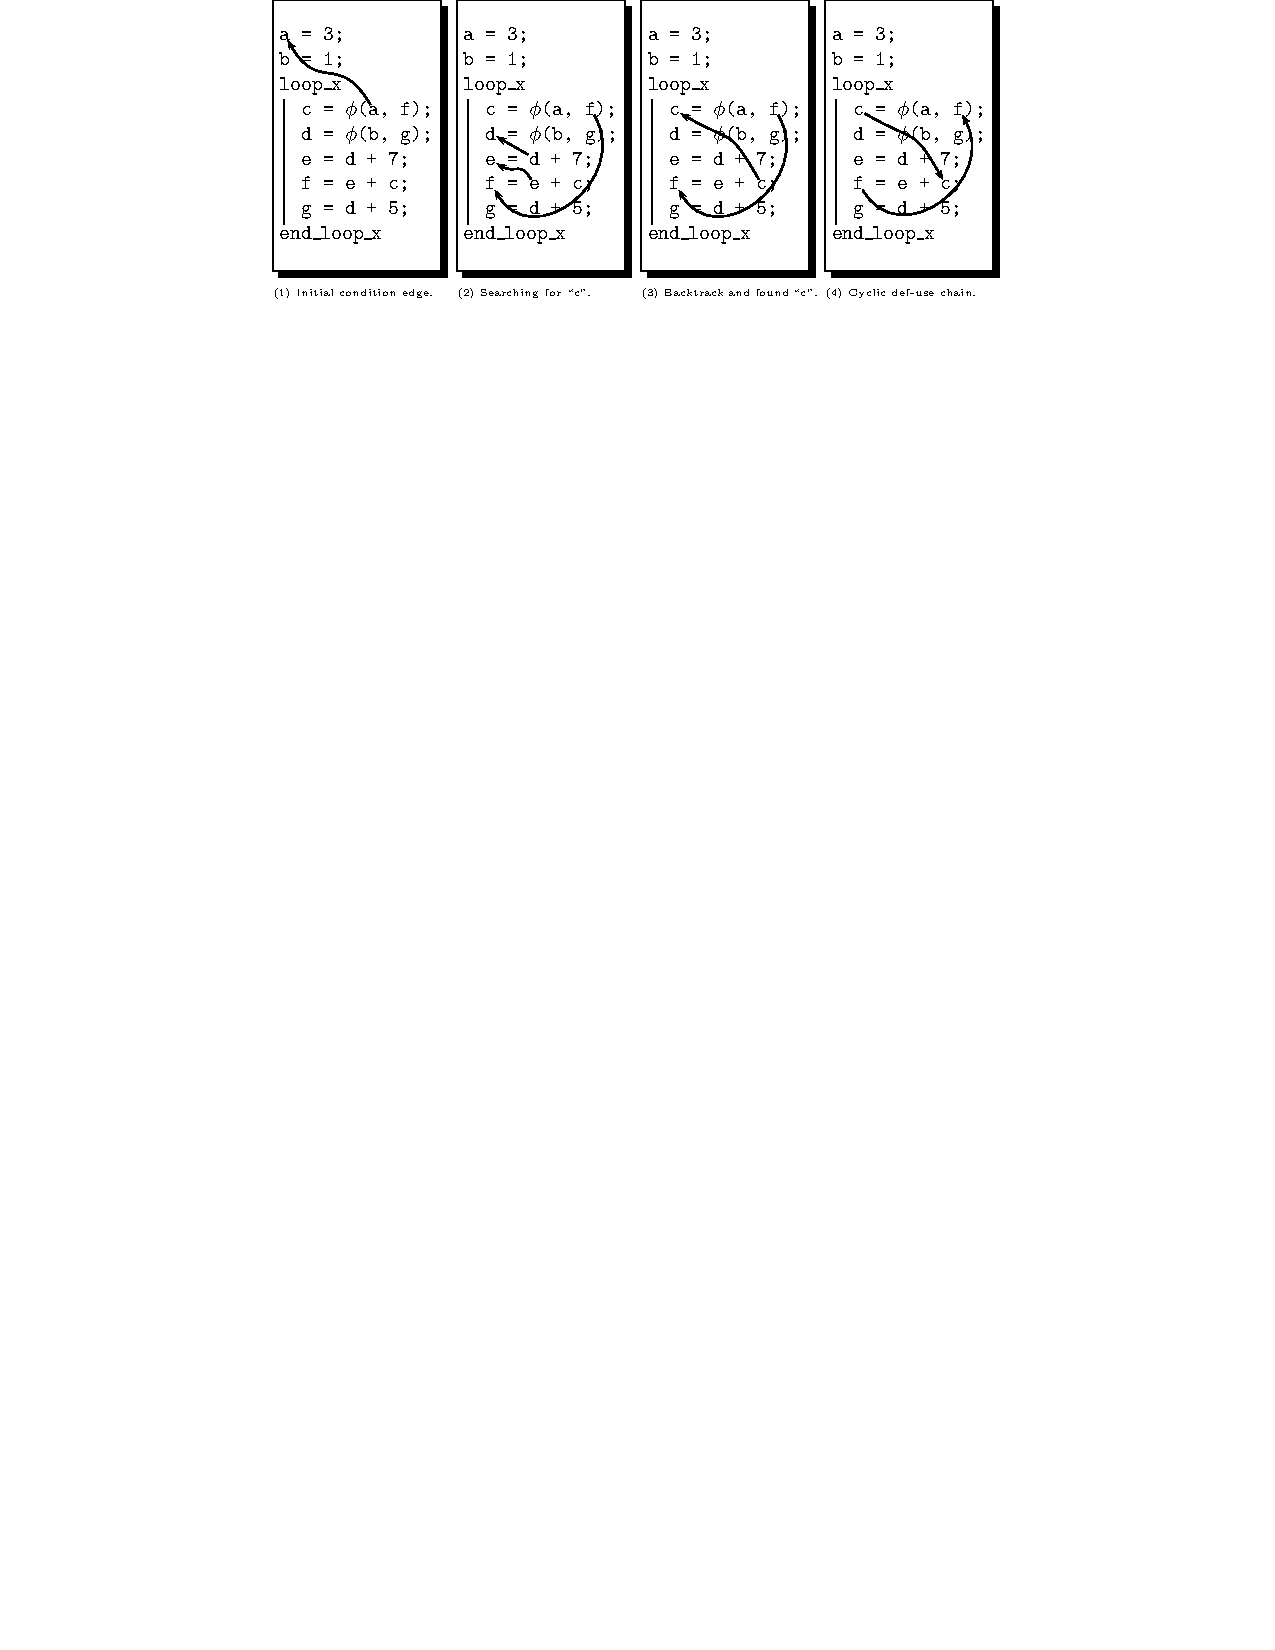
\includegraphics[width=1.2\textwidth]{iv_step}
  \end{center}
  \vspace{-50em}
  \caption{Detection of the cyclic definition.}
  \label{spop:fig:ivstep}
\end{figure}

Let's look at an example, presented in Figure~\ref{spop:fig:ivstep},
to see how this algorithm works.  The arguments of a phi node are
analyzed to determine whether they contain self references or if they
are pointing towards the initial value of the induction variable.  In
this example, (1) represents the edge that points towards the
invariant definition.  When the argument to be analyzed points towards
a longer use-def chain, the full chain is traversed, as shown in (2),
until a phi node is reached.  In this example, the phi node that is
reached in (2) is different to the phi node from which the analysis
started, and so in (3) a search starts over the uses that have not yet
been analyzed.  When the original phi node is found, as in (3), the
cyclic def-use chain provides the step of the induction variable: in
this example, the step is ``+ e''.  Knowing the symbolic expression
for the step of the induction variable may not be enough, as we will
see next, one has to instantiate all the symbols (``e'' in the current
example) defined in the varying loop to precisely characterize the
induction variable.

\subsection{Translation to chains of recurrences}

Once the cyclic def-use chain has been outlined and the overall loop
update expression has been identified, it is possible to translate the
sequence of values of the induction variable to a chain of recurrence.
The syntax of a polynomial chain of recurrence is: $\CHREC{base, +,
  step}_x$, where ``base'' and ``step'' may be arbitrary expressions
or constants, and ``x'' is the loop in which the sequence is
generated.  As a chain of recurrence represents the sequence of values
taken by a variable during the execution of a loop, the semantics of a
chain of recurrence is given by $\CHREC{base, +, step}_x (\ell_x) =
base + step * \ell_x$, that is a function of $\ell_x$ that represents
the number of times the body of loop number $x$ has been executed.

When ``base'' or ``step'' translates to sequences variating in outer
loops, the resulting sequence is represented by a multivariate chain
of recurrences.  For example $\CHREC{\CHREC{0, +, 1}_3, +, 2}_4$
defines a multivariate chain of recurrence with a step of $1$ in loop
number $3$ and a step of $2$ in loop number $4$.

When ``step'' translates into a sequence variating in the same loop,
the chain of recurrence represents a polynomial of a higher degree.
For example, $\CHREC{0, +, \CHREC{4, +, 5}_3}_3$ represents a
polynomial evolution of degree $2$ in loop number $3$.  In this case,
the chain of recurrence is also written omitting the extra braces:
$\CHREC{0, +, 4, +, 5}_3$.  The semantics of the chains of recurrences
is defined, using the binomial coefficients $\binom{n}{p}$, by the
equation:
\begin{equation*}
  \CHREC{c_0,+,c_1,+,c_2,+,\ldots,+,c_n}_k(\vec{\ell})=
  \sum_{p=0}^{n}c_{p}\binom{\ell_k}{p}.
\end{equation*}
with $\vec{\ell}$ the iteration domain vector (the iteration loop
counters for all the loops in which the chain of recurrence variates),
and $\ell_k$ the iteration counter for loop number $k$.  This
semantics allows the rewriting rule:
\begin{equation*}
  \CHREC{c_0, +, \CHREC{c_1, +, c_2}_x}_x = \CHREC{c_0, +, c_1, +, c_2}_x
\end{equation*}
that is very useful in the analysis of induction variables, as it
makes it possible to split the analysis into two phases, with a
symbolic representation as a partial intermediate result:
\begin{itemize}
\item first, the analysis leads to a symbolic form, where the step
  part ``s'' is left in a symbolic form, i.e., $\CHREC{c_0, +, s}_x$;
\item then, by instantiating the step, i.e., $s = \CHREC{c_1, +,
  c_2}_x$, the chain of recurrence is that of a higher degree
  polynomial, i.e., $\CHREC{c_0, +, \CHREC{c_1, +, c_2}_x}_x =
  \CHREC{c_0, +, c_1, +, c_2}_x$.
\end{itemize}

\subsection{Instantiation of symbols and region parameters}

The last step of the induction variable analysis consists in the
instantiation (or further analysis) of symbolic expressions left from
the first step.  This includes the analysis of induction variables in
outer loops, the analysis of the end value of a loop preceding the
analyzed loop, and the replacement of any definitions occurring in
sequence before the loop with their defined expression.  In some
cases, it becomes necessary to leave in a symbolic form every
definition outside a given region, and these symbols are then called
parameters of the region.

Let's look again at the example of Figure~\ref{spop:fig:ivstep} to see
how the sequence of values of the induction variable ``c'' is
characterized with the chains of recurrences notation.  The first
step, after the cyclic definition is detected, is the translation of
this information into a chain of recurrence: in this example, the
initial value (or base of the induction variable) is ``a'' and the
step is ``e'', and so ``c'' is represented by a chain of recurrence
$\CHREC{a, +, e}_1$ that is variating in loop number $1$.  The symbols
are then instantiated: ``a'' is trivially replaced by its definition
leading to $\CHREC{3, +, e}_1$.  The analysis of ``e'' leads to this
chain of recurrence: $\CHREC{8, +, 5}_1$ that is then used in the
chain of recurrence of ``c'', $\CHREC{3, +, \CHREC{8, +, 5}_1}_1$ and
that is equivalent to $\CHREC{3, +, 8, +, 5}_1$, a polynomial of
degree two:
\begin{eqnarray*}
  F(\ell)
  &=& 3\binom{\ell}{0} + 8\binom{\ell}{1} + 5\binom{\ell}{2} \\
  &=& \frac{5}{2}\ell{}^2+\frac{11}{2}\ell + 3.
\end{eqnarray*}

\subsection{Number of iterations and computation of the end of loop value}

One of the important properties of loops is their trip count (i.e.,
the number of times the loop body is executed before the exit
condition becomes true).  In simple loops, the exit condition of the
loop is a comparison of an induction variable against some constant,
parameter, or another induction variable.  The number of iterations is
then computed as the solution of an equation with integer coefficients
and integer solutions, also called a Diophantine equation.  When one
or more coefficients of the Diophantine equation are parameters, the
solution is left under a parametric form.  The number of iterations
can also be an expression variating in an outer loop, in which case,
it can be characterized using a chain of recurrence expression.

With an expression representing the number of iterations in a loop, it
becomes possible to express the evolution functions of scalar
variables variating in outer loops with strides dependent on the value
computed in an inner loop: the overall effect of a loop on a scalar
variable can be computed as an apply of the number of iterations on
the evolution function (of the scalar variable) in the varying loop.

For example, the following code
\begin{verbatim}
x = 0;
for (i = 0; i < N; i++)
  for (j = 0; j < M; j++)
    x = x + 1;
\end{verbatim}
would be written in loop closed \SSA{} form as:
\begin{verbatim}
  a = 0
  b = loop_1_phi (a, c)
  c = close_2_phi (j < M, d)
  d = loop_2_phi (b, d + 1)
  e = close_1_phi (i < N, b)
  i = loop_1_phi (0, i + 1)
  j = loop_2_phi (0, j + 1)
\end{verbatim}
``e'' represents the value of variable ``x'' at the end of the
original imperative program.  The analysis of scalar evolutions for
variable ``e'' would trigger the analysis of scalar evolutions for all
the other variables defined in the loop closed \SSA{} form as follows:
\begin{itemize}
\item first, the analysis of variable ``e'' would trigger the analysis
  of ``i'', ``N'' and ``b''
  \begin{itemize}
  \item the analysis of ``i'' leads to $i = \CHREC{0, +, 1}_1$
  \item ``N'' is a parameter and is left under its symbolic form
  \item the analysis of ``b'' triggers the analysis of ``a'' and ``c''
    \begin{itemize}
    \item the analysis of ``a'' leads to $a = 0$
    \item analyzing ``c'' triggers the analysis of ``j'', ``M'', and ``d''
      \begin{itemize}
      \item $j = \CHREC{0, +, 1}_2$
      \item ``M'' is a parameter
      \item $d = loop\_2\_phi (b, d + 1) = \CHREC{b, +, 1}_2$
      \end{itemize}
    \item $c = close\_2\_phi (j < M, d)$ is then computed as the last value of ``d'' after
      $loop_2$, i.e., it is the chain of recurrence of ``d'' applied
      to the first iteration that does not satisfy $j < M$ and
      because ``j'' counts the number of times the body of $loop_2$
      has run, that is the number of iterations of $loop_2$, i.e.,
      $M$.  So, to finish the computation of the scalar evolution of
      ``c'' we apply ``M'' to the scalar evolution of ``d'', leading
      to $c = \CHREC{b, +, 1}_2 (M) = b + M$;
    \end{itemize}
  \item the scalar evolution analysis of ``b'' then leads to $b =
    loop\_1\_phi (a, c) = loop\_1\_phi (a, b + M) = \CHREC{a, +, M}_1 =
    \CHREC{0, +, M}_1$
  \end{itemize}
\item and finally the analysis of ``e'' ends with $e = close\_1\_phi (i
  < N, b) = \CHREC{0, +, M}_1 (N) = M * N$.
\end{itemize}

The computation of the end of loop value can also be used for
optimization purposes, for example in the case of the constant
propagation or the value range propagation after loops.  It enables
more scalar transformations when the induction variable is used after
its defining loop.  Another interesting use of the end of loop value
is the estimation of the worst case execution time (WCET) where one
tries to obtain an upper bound approximation of the time necessary for
a program to terminate.

\section{Conclusion}
As we have seen in this chapter, the \CFG{} representation is embedded
in the \SSA{} structure, and properties of the \CFG{} like the
execution order and the natural loops can be detected by only looking
at the \SSA{} definitions and uses.  The detection of natural loops is
the first step in the analysis of induction variables: after the
detection of self referent definitions, it is practical to use the
chains of recurrences \cite{BWZ94,KMZ98,Zim01} to characterize the
sequence of values taken by a variable during the execution of a loop.
The number of iterations of loops can be computed based on the
characterization of induction variables.  This paves the way to
advanced loop optimizations that need both the number of iterations
and induction variable characterizations.

